\documentclass[11pt,a4paper,english]{uvamath}
\usepackage[english]{babel}

\usepackage{amsmath, amsfonts, amssymb, a4wide, fancyhdr, lineno, graphicx, epsfig, soul, color, hyperref}
\usepackage[square, numbers]{natbib}

% Running line numbers:
\linenumbers
% Number only every 5:th line:
\modulolinenumbers[5]

%Nodig om een bibliography midden in het artikel te zetten, ipv aan het einde zoals eigenlijk gebruikelijk is
\renewcommand{\bibsection}{}

% TODO command
\newcommand{\todo}[1]{
    \hl{#1}
}

% The things that should be filled in by each group, depending on their situation, are written in a todo command, \todo{like this text}. All text in normal the normal font, is applicable for any group. However, everyone is free to adapt any text, and it is even suggested to look at all text critically and make changes if needed.

% Project specific commands
\author{Tom van Duist \& Kevin van den Bekerom}

\newcommand{\projectname}{\todo{Project Name}\ }


\newcommand{\aanpassen}[1]{ {\sethlcolor{green} \hl{#1}} }

\title{Requirements Document}
%Variables
\newcommand{\TitelAbbr}{RD}
\newcommand{\Version}{0.1}



\what{Lab assignment Requirements Engineering}
\supervisors{}
\author{Tom van Duist \& Kevin van den Bekerom}



\begin{document}

\maketitle


\tableofcontents

\chapter*{Document Status Sheet}
\section*{Document status overview}
\subsection*{General}
\begin{tabular}[!]{ll}
    Document title:     & Architectural Design Document\\
    Authors:           	& Kevin van den Bekerom \\ 
						& Tom van Duist \\
    Document status:    & Draft release\\
\end{tabular}

\subsection*{Document history}
\begin{tabular}[!]{|l|l|l|l|}
    \hline
    \emph{Version}    &   \emph{Date} &  \emph{Reason of change}\\
    \hline
    0.0 & 02-09-2015 &  Setup of the document layout\\    
    \hline
    0.1 & 29-10-2015 & Release version week 1 \\
    \hline
\end{tabular}

\clearpage

%\section*{Document Change Records since previous issue}
%\subsection*{General}
%\begin{tabular}[!]{ll}
%   Datum:          &   2015-06-09 \\
%    Document title: &   Architectural Design Document (ADD)\\
%    Identification:  &   \TitelAbbr\_\Version.pdf\\
%\end{tabular}

%\subsection*{Changes}
%\begin{tabular}[!]{|l|l|p{8 cm}|}
%    \hline
%    \emph{Chapter} &   \emph{Paragraph}    &   \emph{Reason to change}\\
%    \hline
%    \ref{c:main_fun} &  whole chapter      & Make prioritizing clear using Moscov model. Clarified functionalities. \\
%    \hline
%    dfdf& tt & ff. \\
%    \hline
%\end{tabular} 

%\chapter{Introduction}
%Blabla.

\chapter{Project Plan}
The project plan for the first four weeks is explained in this chapter. The goal is to discover some of the essential features that should be provided by the successor of Blackboard. We base our project plan on the requirements engineering process, see Figure \ref{fig:spiral_model} \cite{RE_book} (chapter 1.1.6). This book identifies four phases of requirements engineering; 

\begin{enumerate}
	\item Domain understanding and elicitation.
	\item Evaluation and negotiation.
	\item Specification and documentation.
	\item Quality assurance.
\end{enumerate}

During the first week we will get familiar with the problem world, as described in the first phase \cite{RE_book}. We will investigate the system-as-is, ourselves, and ask users (students) about their experiences. We will work trough the questions listed in the relevant section in the book. We will also compose a list of stakeholders, which we interview in the coming weeks.

Week 2 will resolve around the second phase: evaluation and negotiation. The goal of this week is to find all critical (business) goals of the stakeholders of the system. Why is it replaced? What is the relation to the mission and vision of the UvA (if there is any)? Why did the UvA use an education management tool in the first place? What are the goals of the students in relation to the tool etc. During this week we will interview remaining stakeholders, to verify and add upon the information we gathered in the first week. We will also interview more students with prepared questions.

During week 3 we will draft an initial set of requirements. After week 3 the first draft version of the Requirements Document is finished. We will focus on the smallest set of requirements that together realize the business goals on an acceptable level, due to limited time. 

In week 4 we will plan meetings with relevant stakeholders to asses the set of requirements we drafted for the new system. Assessment focuses on whether we forgot crucial requirements and if the requirements are consistent.  

Note that we conduct one round of the spiral model, see Figure \ref{fig:spiral_model}. There will be some backtracking to other phases (previous weeks), because some information becomes available after the relevant week/phase. 

\begin{figure}[h]
	\centering
	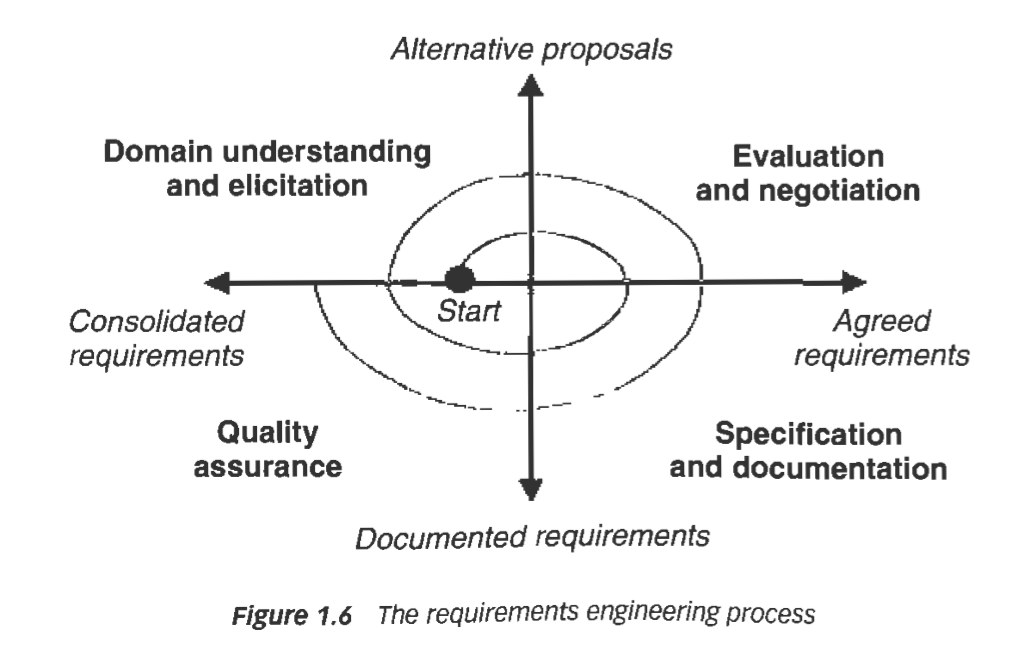
\includegraphics[width=0.75\linewidth]{images/re_process}
	\caption{Spiral Model of requirements engineering process}
	\label{fig:spiral_model}
\end{figure}



\chapter{Domain Analysis}
In the first week we focused on getting a better understanding of the domain in order to form a better understanding of the problems in the domain with relation to the goals, which we will gather during the next phase.

\section{Glossary of terms}
\todo{List all relevant terms in the problem world}

\section{Organization}
The organization in which Blackboard is used is the University of Amsterdam (UvA). 

The organization within which the system-as-is takes place: its structure, strategic objectives,
business policies, roles played by organizational units and actors, and dependencies
among them.

\section{Goal}
The goal of a requirement engineering project in a perfect world would be strife to find all of most important quality requirements for all relevant stakeholders. As stated in Contextual Design \cite{contextual_design} a design process could always be further elaborated, so finding all and every requirements for all stakeholders is an illusion.

Because of this and the time constraints of this project, the goal will be limited to the following: \emph{find a couple of the major requirements for the main stakeholder(s)}. We believe this is measurable enough for the assignment given the time frame but still enough of an abstraction given that we do not yet have a clear enough understanding of the domain at this time to make it more concrete without taking away from the achieveability.

\section{Scope}
The scope of the system-as-is: its underlying objectives, the components forming it, the
concepts on which it relies, the tasks involved in it, the information flowing through it,
and the constraints and regulations to which the system is subject.

\section{Stakeholders}
\begin{itemize}
	\item Users: Both students and teachers
	\item Management:
	\item Blackboard (company):
\end{itemize}

The set of stakeholders to be involved in the RE process.

\section{Strengths and Weaknesses}
Students:
\begin{itemize}
	\item[+] Easy way to access course specific information.
	\item[+] Latest schedule of course.
	\item[-] Hard to use in the beginning.
	\item[-] Only marginal functionality used, e.g. "We \textit{have} to use it."
\end{itemize}

The strengths and weaknesses of the system-as-is, as perceived by the identified stakeholders.

\section{Domain facts}
The following facts are from a study in \cite{ict_study}. The implications for the requirements engineering process are in italic.
\begin{itemize}
	\item Formative feedback can help students improve their work. \textit{BB does not offer formative feedback, this is merely a responsibility of the teacher.}
	\item Should be clear link between learning goals (of a course) and the ICT solution. If the ICT solution is merely a means to reach a goal it will not improve learning. 
	\item Important how ICT is used that determines its effectiveness. \textit{If a domain fact is that students use BB because they have to, then a BB-related solution might not be effective.}
	\item Teachers use ICT based on their own skills. This might undermine its effectiveness.
	\item ICT changes rapidly. Partly, but in an increasingly lesser manner, by Moore's Law. In week 3 we will investigate this fact more in the literature.
	\item The availability of a tool does not determine its effectiveness. In its initial stages the focus is on how to use the tool, rather than using the tool for learning-promoting purposes.
	\item Research also rarely reports on technical issues or problems with equipment, yet these are what teachers find act as barriers to increasing the use of technology in classrooms.
	\item Media reports faster on trends then research can validate or discredit using that technology. Example: Interactive Whiteboards. 
	\item ICT does not help increase pupils attainment.
\end{itemize}



\chapter{Essential stakeholder goals}\label{stakeholder_goals}
During this phase we set out to gather the essential stakeholder goals. Each stakeholder has a specific goal, be it something that has to do with the system or something entirely different. Our aim is to identify these goals in order to understand how the ELE of the UvA can assist in reaching these goals and which minimal features are needed to this end.

\section{UvA}
Taken from the core values of the UvA is the following: \\
\textit{Engagement for the UvA and its staff implies the age-old obligation – based on a privileged academic position – to use acquired knowledge and insights to play an ongoing, prominent and visible role in the social debate. This value also reveals that the UvA is committed to the maximum development of the individual talents of its staff and students. Additionally, the choice of this core value suggests a strong mutual involvement between students, staff, employees, study programmes, institutes and the institution as a whole. And, lastly, there is an important link between academia and society. The UvA is located in historical and modern buildings throughout the city of Amsterdam, thus making it an integral part of the city.}

Important goals are:
\begin{enumerate}
	\item The UvA is committed to the maximum development of the individual talents of its staff and students.
	\item The UvA strives for a strong mutual involvement between students, staff, employees, study programs, institutes and the institution as a whole.
\end{enumerate}

\section{Teacher}
Taken from the UvA goal and by talking to teachers.
\begin{enumerate}
	\item Develop individual skills.
	\item Convey knowledge to students.
\end{enumerate}

\section{student}
The student goals still need to be confirmed by finding a relevant paper. We believe these are the broad categories of students:
\begin{enumerate}
	\item Optimally develop one's personal and academic skills.	
	\item Obtain diploma.
\end{enumerate}



\chapter{Domain questions ofzo?}
In order to find the essential features of an ELE we set out to find how an ELE can support the various stakeholders with achieving their goals. To this end we have some questions for which we want to find the answers. This we will do by conducting research and elicitations amongst the various stakeholders.

Following is a list questions, loosely ordered on importance:
\begin{itemize}
	\item What are the essential features of the Blackboard (or similar ELE) system for the UvA?

	\item To what extend does the current Blackboard system support the UvA goals?
	\begin{itemize}
		\item To what extend does the current system support the goals of the teachers?
		\item To what extend does the current system support the goals of the students?
	\end{itemize}
	
	\item Which type of usability problems have no impact on education?
	\item What characteristics of users are important to consider for the selection of a new system?
	\item How will the new Blackboard system contribute to the goals of the UvA?
\end{itemize}

In this chapter we will answer these questions (though we may not be able to answer them all) and update the information once we get new data. We will also note how reliable the information is based on the source and/or frequency of the information.


\section{What are the essential features of the Blackboard (or similar ELE) system for the UvA?}
In order to find the essential features of the Blackboard system we have performed elicitations amongst both teachers and students. From these we have devised the following preliminary list of essential features:

\begin{itemize}
	\item Teacher:
	\begin{itemize}
		\item Publishing documents
		\item Publishing assignments
		\item Publishing announcements
	\end{itemize}

	\item Student:
	\begin{itemize}
		\item Retrieve relevant information/documents.
		\item Hand in digital assignments.
	\end{itemize}
\end{itemize}

We can distil this into a single feature list:
\begin{itemize}
	\item Share documents.
	\item Hand in digital assignments.
	\item Publish announcements.
\end{itemize}

\subsection{Reliability}
We deem this preliminary feature list as quite reliable and representative for the essential use of Blackboard by teachers and students. The sources of this information are the elicitations that we performed but also our own experience, and talking to the users (students and teachers).

This list is not very reliable for the representativeness for the features with regards to the goals of the UvA, to answer that part of the question we first need to reliably answer the following question "\emph{\ref{uva_goal_question}: \nameref{uva_goal_question}}".
\todo{update when answered}


\section{To what extend does the current Blackboard system support the UvA goals?} \label{uva_goal_question}
In order to answer this question we have divided it into two sub-questions. As the main goal of the UvA (see \ref{stakeholder_goals}: \nameref{stakeholder_goals}) could be divided into sub-goals for its staff and students we have done the same with this question to make it easier to answer.

\subsection{To what extends does the system support the goals of the teachers?}
By reasoning about how teachers develop their skills, from personal experience by looking around in the UvA and talking to teachers we can answer this question for the staff:
\begin{itemize}
	\item Teachers do not develop their skills through Blackboard, they develoop their skills by performing activities related to their field. For example by developing assignments for students. Or by doing personal research, read papers, go to conferences etc.
\end{itemize}

\subsection{To what extends does the system support the goals of the students?}
By talking to teachers we have answered this question for students:
\begin{itemize}
	\item Students do not develop their skills through Blackboard because the system does not create \emph{good} teachers. Students develop their skills through individual discipline and programs set up by competent teachers, Blackboard is just one of the many tools used by the teachers. It still boils down to the teacher himself to channel his knowledge.
\end{itemize}

\subsection{Reliability}
Because our sample size for both answers is really low, and both teachers and ourself are just talking about personal experiences and beliefs this is not a reliable answer. We might be able to confirm it by doing proper research. \todo{research}

We might also get a more reliable (and possibly different) answer by substituting the main question by two other questions:
\begin{itemize}
	\item Does Blackboard save the teachers time?
	\item Will teachers who spend (relatively) less time on bureaucracy teach better?
\end{itemize}


\section{Which type of usability problems have no impact on education?}
From our elicitations with and talking to students we learned:
\begin{itemize}
	\item The usability problems that are usually connected to Blackboard have no impact on the	education. All who reported usability problems also stated that it was really annoying in the first couple of weeks, but after they got used to it the problem almost	entirely ceased to exist.
\end{itemize}

\subsection{Reliability}
The reliability of these statements is very doubtful. As we later learned from reading Thinking, Fast and Slow by Kahneman, people are not eager to open up and possibly embarrass themselves. So they might not let us know that they find Blackboard hard to use, at it might show that they personally do not have the skills to use the tool, which they can experience as embarrassing.

To answer this question more reliable we might substitute the questions regarding usability by different questions, which are not directed personally at the interviewee, but are harder for him to answer. As Kahneman showed, in his mind the interviewee will (unconsciously) substitute the question by looking at his own experience (and of people around him), which is the answer that we are looking for. \todo{perform elicitaion with substitude questions}


\section{What characteristics of users are important to consider for the selection of a new system?}
To answer this question we first set out to find different characteristics of users through our elicitations, focusing mainly on their study goals and use of resources to this end. What we encountered was not really what we expected. Obviously all students want to pass their exams and eventually earn a degree, but besides this most students want to develop specific skills, broaden or deepen their knowledge base; earn intrinsic knowledge to some degree. What we found was:
\begin{itemize}
	\item Irrespective of the degree of intrinsic knowledge the student seeks, he uses other sources of information than those solely provided by their teacher (be in through Blackboard or other means).
\end{itemize}

So we found that irrespective of the characteristics regarding study goals of the student, he independently uses resources outside of the ELE to get additional information to help achieve these goals.

\subsection{Reliability}
Again our sample size is small, but the results were not really what we expected. Because of this we believe the information more reliable than when it merely confirmed our predisposition as it is less likely that we were suggestive of the answer during our elicitation.

Finding some proper research to back up our results would strengthen the reliability of the conclusion. \todo{research}


\section{How will the new Blackboard system contribute to the goals of the UvA?}
As we found out when answering "\emph{\ref{uva_goal_question}: \nameref{uva_goal_question}}", we doubt if the current system has a notable contribution towards the main goal of the UvA and are not sure if such a system ever will, although this is hard to answer.

Another very specific goal of the UvA that we found states:
	\todo{state the goal + reference}
Because this goal is very specific about the IT systems used within the university it should be met by the new Blackboard system. Otherwise it should not be chosen in the first place.


\chapter{References}

\begin{thebibliography}{9}
	
	\bibitem{contextual_design}
	Hugh Beyerand and Karen Holtzblatt,
	\emph{Contextual Design},
	
	\bibitem{RE_book}
	Axel van Lamsweerde,
	\emph{Requirements Engineering: From System Goals to UML Models to Software Specifications}
	
	\bibitem{ict_study}
	Steve Higgins,
	\emph{Does ICT improve learning and teaching in schools},
	Newcastle University.
	
	\bibitem{uva_mission}
	UvA mission \\
	\url{https://www.uva.nl/en/about-the-uva/uva-profile/mission-and-identity/core-values-and-ambitions/core-values-and-ambitions.html}
	
\end{thebibliography}


\appendix


\end{document}
